\begin{figure}
	\begin{center}
		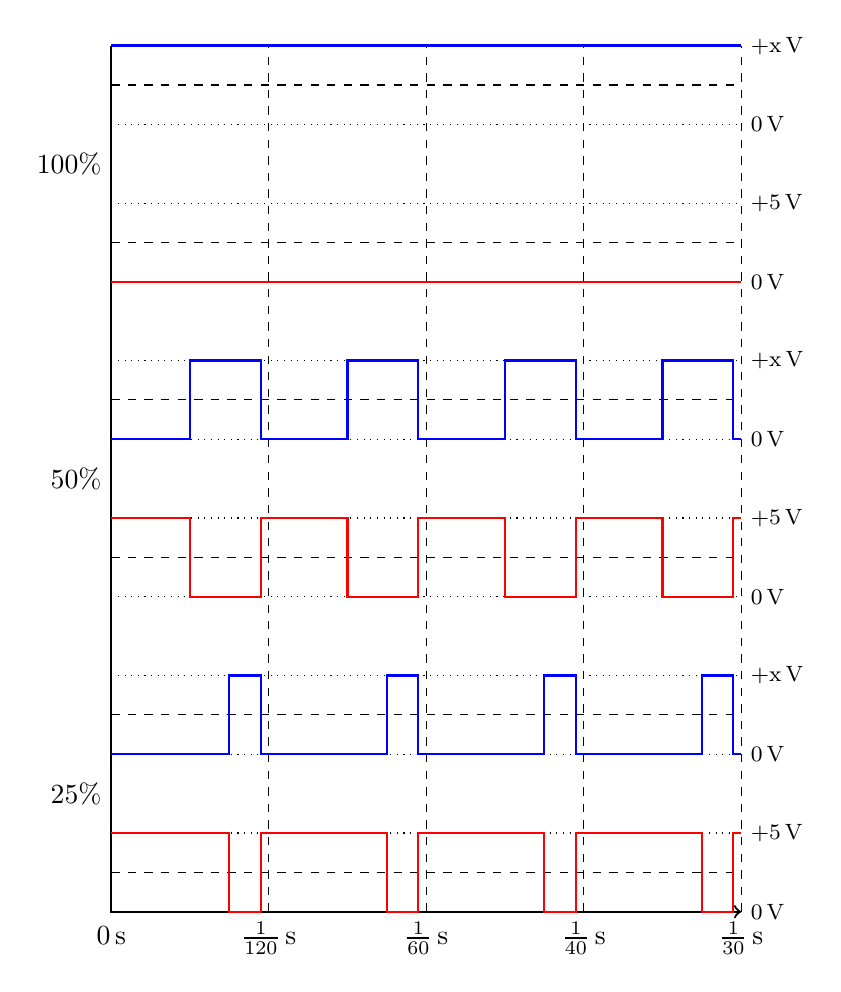
\begin{tikzpicture}[scale=.5]
			\draw [thick, <-] (16,0) -- (0,0) -- (0,22);
			\foreach \x in {4, 8, 12, 16} {
				\draw [dashed] (\x,0) -- (\x,22);
			}
			\foreach \y in {0, 4, 8, 12, 16, 20} {
				\draw [dotted] (0,\y) -- (16,\y);
				\draw [dotted] (0,\y+2) -- (16,\y+2);
				\draw [dashed] (0,\y+1) -- (16,\y+1);
			}
			\foreach \y in {0, 8, 16} {
				\node [right] at (16,\y+2) {\footnotesize +5\,V};
				\node [right] at (16,\y) {\footnotesize 0\,V};
				\node [right] at (16,\y+4) {\footnotesize 0\,V};
				\node [right] at (16,\y+6) {\footnotesize +\Var{x}\,V};
			}
			\node [left] at (0,3) {25\%};
			\node [left] at (0,11) {50\%};
			\node [left] at (0,19) {100\%};
			\node [below] at (0,0) {\vphantom{$1\over1$}0\,s};
			\node [below] at (4,0) {$1\over120$\,s};
			\node [below] at (8,0) {$1\over60$\,s};
			\node [below] at (12,0) {$1\over40$\,s};
			\node [below] at (16,0) {$1\over30$\,s};

%			\draw [thick,red] (0,2) -- (16,2);
			\draw [thick,red] (0,2) -- (3,2) -- (3,0) -- (3.8,0) -- (3.8,2) --
					  (4,2) -- (7,2) -- (7,0) -- (7.8,0) -- (7.8,2) --
				          (8,2) -- (11,2) -- (11,0) -- (11.8,0) -- (11.8,2) --
				          (12,2) -- (15,2) -- (15,0) -- (15.8,0) -- (15.8,2) --
				 	  (16,2);
			% 0 1 2 -> 6 5 4
			\draw [thick,blue] (0,4) -- (3,4) -- (3,6) -- (3.8,6) -- (3.8,4) --
					  (4,4) -- (7,4) -- (7,6) -- (7.8,6) -- (7.8,4) --
				          (8,4) -- (11,4) -- (11,6) -- (11.8,6) -- (11.8,4) --
				          (12,4) -- (15,4) -- (15,6) -- (15.8,6) -- (15.8,4) --
				 	  (16,4);
			\draw [thick,red] (0,10) -- (2,10) -- (2,8) -- (3.8,8) -- (3.8,10) --
				          (4,10) -- (6,10) -- (6,8) -- (7.8,8) -- (7.8,10) --
				          (8,10) -- (10,10) -- (10,8) -- (11.8,8) -- (11.8,10) --
				          (12,10) -- (14,10) -- (14,8) -- (15.8,8) -- (15.8,10) --
				 	  (16,10);
			% 8 9 10 -> 14 13 12
			\draw [thick,blue] (0,12) -- (2,12) -- (2,14) -- (3.8,14) -- (3.8,12) --
				          (4,12) -- (6,12) -- (6,14) -- (7.8,14) -- (7.8,12) --
				          (8,12) -- (10,12) -- (10,14) -- (11.8,14) -- (11.8,12) --
				          (12,12) -- (14,12) -- (14,14) -- (15.8,14) -- (15.8,12) --
				 	  (16,12);
			\draw [thick,red] (0,16) -- (16,16);
			\draw [thick,blue] (0,22) -- (16,22);
		\end{tikzpicture}
		\caption{\label{fig:dcdutycycle}Duty Cycles of Logic (red) and DC SSR Outputs (blue)}
	\end{center}
\end{figure}
